\documentclass[a4paper,12pt]{article}
%%%%%%%%%%%%%%%%%%%%%%%%%%%%%%%%%%%%%%%%%%%%%%%%%%%%%%%%%%%%%%%%%%%%%%%%%%%%%%%%%%%%%%%%%%%%%%%%%%%%%%%%%%%%%%%%%%%%%%%%%%%%%%%%%%%%%%%%%%%%%%%%%%%%%%%%%%%%%%%%%%%%%%%%%%%%%%%%%%%%%%%%%%%%%%%%%%%%%%%%%%%%%%%%%%%%%%%%%%%%%%%%%%%%%%%%%%%%%%%%%%%%%%%%%%%%
\usepackage{eurosym}
\usepackage{vmargin}
\usepackage{amsmath}
\usepackage{graphics}
\usepackage{epsfig}
\usepackage{subfigure}
\usepackage{fancyhdr}
\usepackage{listings}
\usepackage{framed}
\usepackage{graphicx}
\usepackage{amsmath}
\usepackage{chngpage}
%\usepackage{bigints}


\setcounter{MaxMatrixCols}{10}
%TCIDATA{OutputFilter=LATEX.DLL}
%TCIDATA{Version=5.00.0.2570}
%TCIDATA{<META NAME="SaveForMode" CONTENT="1">}
%TCIDATA{LastRevised=Wednesday, February 23, 2011 13:24:34}
%TCIDATA{<META NAME="GraphicsSave" CONTENT="32">}
%TCIDATA{Language=American English}

%\pagestyle{fancy}
%\setmarginsrb{20mm}{0mm}{20mm}{25mm}{12mm}{11mm}{0mm}{11mm}
%\lhead{MA4413} \rhead{Mr. Kevin O'Brien}
%\chead{Statistics For Computing}
%\input{tcilatex}

\begin{document}
\begin{center}
       
\includegraphics[scale=0.55]{shieldtransparent2}
\end{center}

\begin{center}
\vspace{1cm}
\large \bf {FACULTY OF SCIENCE AND ENGINEERING} \\[0.5cm]
\normalsize DEPARTMENT OF MATHEMATICS AND STATISTICS \\[1.25cm]
\large \bf {MID-SEMESTER ASSESSMENT} \\[1.5cm]
\end{center}

\begin{tabular}{ll}
MODULE CODE: MA4128 & SEMESTER: Spring \\[1cm]
MODULE TITLE: Advanced Data Modeling & DURATION OF EXAM: 1 hour \\[1cm]
LECTURER: Mr. Kevin O'Brien & GRADING SCHEME: 50 marks \\
& \phantom{GRADING SCHEME:} \footnotesize {20\% of module grade} \\[0.8cm]
\\[1cm]
\end{tabular}
\begin{center}
{\bf INSTRUCTIONS TO CANDIDATES}
\end{center}

{\noindent \\ Scientific calculators approved by the University of Limerick can be used. \\
Statistical tables provided at the end of the exam paper.\\
Students must attempt ALL questions}
\newpage



% - Section 1 Inference Procedures
        % a. Parametric
        % b. Non Parametric
% - Section 2 Linear Models
        % a. SLR
        % b. MLR
% - Section 3 Linear Models
        % a. Robust Regression
        % b. AIC
% - Section 4 Statistical Process control
        % a. Control Limits
        % b. Theory Questions
        % c. Interpreting Charts
        % d. CUSUM and ARL
% - Section 5 Experimental Design 1
        % a. Definitions for ED
        % b. One Way ANOVA
% - Section 6 Experimental Design 2
        % a.
        % b.


\subsection*{Question 1. (10 marks) Nelson Rules for Control Charts}
% \subsection*{Question 47 - Nelson Rules for Control Charts}
The \textbf{Nelson Rules} are a set of eight decision rules for detecting ``out-of-control" or non-random conditions on control charts. These rules are applied to a control chart on which the magnitude of some variable is plotted against time. The rules are based on the mean value and the standard deviation of the samples.\\

\begin{itemize}
	\item[(i)] ($4 \times 2.5$ Marks) Discuss any four of these rules, and how they would be used to detect ``out of control" processes. Support your answer with sketches.
\end{itemize}

\bigskip 
\begin{framed}
	\noindent \textit{In your answer, you may make reference to the following properties of the Normal Distribution. Consider the random variable $X$ distributed as
		\[X \sim \mathcal{N}(\mu,\sigma^2)\]
		where $\mu$ is the mean and $\sigma^2$ is the variance of an random variable $X$.}
	\begin{itemize}
		\item $\Pr( \mu - 1\sigma \leq X \leq \mu + 1\sigma ) = 0.6827$
		\item $\Pr( \mu - 2\sigma \leq X \leq \mu + 2\sigma ) = 0.9545$
		\item $\Pr( \mu - 3\sigma \leq X \leq \mu + 3\sigma )= 0.9973$
		
	\end{itemize}
\end{framed}
\noindent \textit{Marking Scheme: For Each Rule: A statment of the the rule is worth 1 Mark. A derviation of the probability is worth 1 Mark. A Sketch is worth 0.5 Marks}.
\newpage
%--------------------------------------------------------------------------------------------------------%


\newpage
\subsection*{Question 2. (10 marks) Binary Classification }
%\subsection*{Question 4. (20 marks) }
\begin{itemize}
	\item[(a)]  \textbf{\textit{ROC Curves	(4 Marks) }}\\
	What is a ROC curve? Explain its function, how it is determined, and the means of interpreting the curve. Support your answer with a sketchs.
\end{itemize}
\bigskip

\begin{itemize}
	\item[(b)] \textbf{\textit{Performance Metrics (6 Marks)}}\\
	For following binary classification outcome table, calculate the following appraisal metrics.
	\begin{itemize}	
		\item[(i.)] (1 Mark)	Accuracy;
		\item[(ii.)] (1 Mark)	Recall;
		\item[(iii.)] (1 Mark)	Precision;
		\item[(iv.)] (1 Mark)	F-measure.
	\end{itemize}	
	\vspace{-0.6cm}
		\begin{center}
		\begin{tabular}{|c|c|c|}
			\hline  & \phantom{spa}Predict Negative\phantom{spa} & \phantom{spa}Predict Positive\phantom{spa} \\ 
			\hline\phantom{spa} Observed Negative \phantom{spa}&	9600	&	20	\\ 
			\hline \phantom{spa}Observed Positive\phantom{spa} & 	300	&	80	\\ 
			\hline 
		\end{tabular} 
	\end{center}
	
	\begin{itemize}	
		\item[(v.)] (2 Marks) Explain why the F-measure is considered a more informative measure of performance than the Accuracy score.
		%	\item[(iii.)](2 Marks) Define Specificity and Sensitivity. You make reference to previous answers.
	
	\end{itemize}
\end{itemize}






%-------------------------------Start of Question 2A%
\newpage



\newpage









%%-------------------------------------%
%\subsection*{Question 3. (20 marks) Multiple Linear Regression Models }
%\begin{itemize}
%
%\item[(a)] Explain the following terms:
%\begin{itemize}
%\item[i.] (2 marks) Over-fitting,
%\item[ii.] (2 marks) Multicollinearity,
%\item[iii.] (2 Marks) Heteroscedascity.
%\end{itemize}
%\item[(b)] Answer the following questions related to model selection techniques for linear models.
%\begin{itemize}
%\item[i.] (2 marks) Explain why the adjusted $R^2$ value may differ in value from the corresponding multiple $R^2$ value for the same fitted model.
%\item[ii.] (2 marks) Explain how the \emph{Akaike information criterion} would used to compare two models fitted for the same data.
%\end{itemize}
%
%\item[(c)]
%In an experiment to determine hydrolysable tannins in plants by absorption spectroscopy, the following results from ten samples were obtained and are tabulated below. A simple linear regression model, predicting absorbance values using concentration as the independent variable, was fitted to the data.
%
%
%%Absorbance= c(0.084, 0.183, 0.326, 0.464, 0.643, 0.707, 0.717, 0.734 ,0.749 ,0.732) ;
%%Concentration= c(0.123, 0.288, 0.562, 0.921, 1.420, 1.717, 1.921, 2.137 ,2.321, 2.467) ;
%%plot(Concentration,Absorbance,pch=18,col="red",font.axis=2,font.lab=2)
%%abline(coef(lm(Absorbance~Concentration)))
%%
%%Conc.Squared = (Concentration^2)
%%Conc.Cubed = (Concentration^3)
%%ModelA = lm(Absorbance~Concentration)
%%ModelB = lm(Absorbance~Concentration+Conc.Squared)
%%ModelC = lm(Absorbance~Concentration+Conc.Squared+Conc.Cubed)
%
%\begin{center}
%\begin{tabular}{|c||c|c|c|c|c|}
%  \hline
%  % after \\: \hline or \cline{col1-col2} \cline{col3-col4} ...
%Sample & 1 & 2 & 3 & 4 & 5 \\ \hline
%Absorbance & 0.084& 0.183& 0.326& 0.464& 0.643\\
%Concentration & 0.123& 0.288& 0.562& 0.921& 1.420\\ \hline
%Sample & 6 & 7 & 8 & 9 & 10 \\ \hline
%Absorbance & 0.707& 0.717& 0.734 &0.749 &0.732\\
%Concentration & 1.717& 1.921& 2.137 &2.321&2.467\\
%  \hline
%\end{tabular}
%\end{center}
%
%\begin{center}
%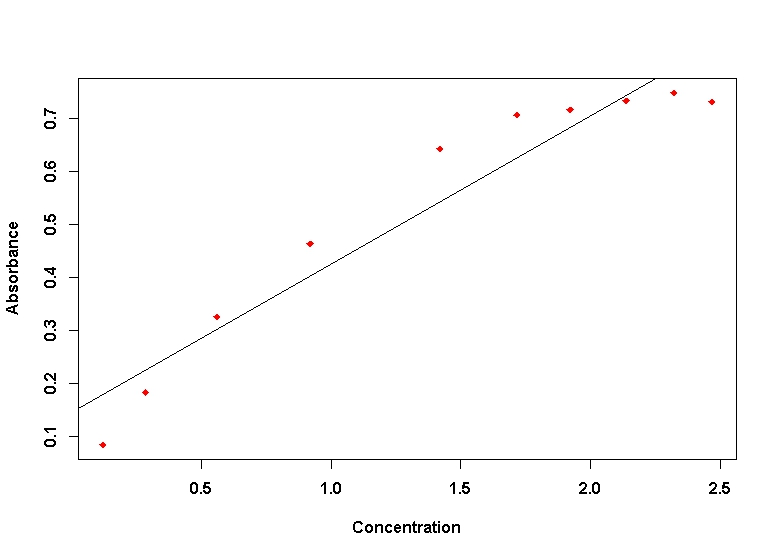
\includegraphics[scale=0.55]{ExamQ3plot}
%\end{center}
%
%
%\begin{itemize}
%\item[i.] (2 marks) Is the simple linear regression model approach suitable for this study? Explain your answer with reference to the scatter-plot.
%%\item[ii] (2 marks) Two polynomial models were also fitted to the data. Description of all three fitted models are found in the three blocks of \texttt{R} code below. The \emph{Akaike information criterion} is also listed, for each of the three fitted models.
%\end{itemize}
%
%
%
%\item[(d)] 
%
%%\end{document}
%--------------------------------------------------------%

\subsection*{Question 3. (10 marks) Hierarchical Clustering}


\begin{itemize}
		\item[(i.)](1 Mark)  Compute the Euclidean distance between the following points.
		\[ A = \c(4,6,8,2)\]
		\[ B = \c(3,6,1,6)\]
%		
%	\item[(i.)](2 Marks) What is the purpose of a cluster analysis?
	
%	\item[ii.](2 Marks)  A discriminant analysis is similar to a cluster analysis; however, there is one fundamental difference.  Explain this difference.
	
	\item[(ii.)](2 Marks) Why do you standardize variables before carrying out a cluster analysis.
		Explain why using the standardized value may not be suitable in some cases? Give another example of numeric transformation. 
	%What is the difference between a linkage method and a distance measure?
	
	\item[(iii.)](4 Marks)  Compare and contrast any three linkage methods. Support your answer with sketches
	
	\item[(iv.)](1 Mark)  In the context of hierarchical cluster analysis, distinguish between agglomerative clustering and divisive clustering.
	%	\item[ix.](2 Marks)  What is a vertical icicle plot used for? Give a brief description, supporting your answer with sketches.

	
	
	\item[(v.)](2 Marks)  How do we determine the appropriate number of clusters?  Give two different visualization methods that are used to display the outcome of a cluster analysis.
	
%	\item[vi.](2 Marks) Standardization
%	
%	\item[vii.](2 Marks)  Explain the difference between Ward's method and k-means
%	clustering.
%	%\item[7.] Vertical Icicle Plot


	
\end{itemize}



%-----------------------------------------------------------%
\newpage

\subsection*{Question 4. (10 marks) K-Means Clustering}

\begin{itemize}
	\item[(i.)] (5 Marks) Explain the process of k-means clustering, starting with initial cluster allocation. You may work on the basis of a two-cluster solution. Support your answer with several sketches.
	\item[(ii.)] (2 Marks) Compare and contrast k-means clustering and hierarchical clustering in terms of the number of cluster determined.
	\item[(iii.)] (3 Marks) For a 4 cluster solution, Interpret the ANOVA table below.
\end{itemize}


\begin{figure}[h!]
\centering
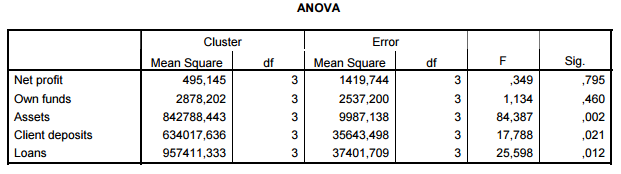
\includegraphics[width=1.1\linewidth]{ANOVA}
\end{figure}


%-----------------------------------------------------------------%
\newpage

\subsection*{Question 5. (10 marks) Modelling Count Variables }


\begin{itemize}
	\item[(i.)] (2 Marks)
	What is Poisson regression used to model. State any assumptions that must be checked before it can be used as an analysis.
%	Poisson Processes and Count Variables
%	Be able to give some examples
%	Checking 
%
%	Simulation Studies to Check range of ratio values to be expected.
	
	\item[(ii.)] (1 Mark) The \texttt{R} Code output given below is used to predict the number of awards won by students. \begin{itemize} 
		\item[$\bullet$] Information is provided on which of the three school programs the student takes part in (\textit{General}, \textit{Vocational} or \textit{Academic}). 
		\item[$\bullet$] Also we are given the mathematics test score.
		\end{itemize}
		State the mathematical formula used to predict the numer of awards won.\\
\textit{You can denote \textbf{progAcademic}, \textbf{progVocational} and \textbf{math} as $x_1$,$x_2$ and $x_3$ respectively.}


\begin{framed}
\begin{verbatim}
Coefficients:
               Estimate Std. Error z value Pr(>|z|)    
(Intercept)     -5.2471     0.6585   -7.97  1.6e-15 ***
progAcademic     1.0839     0.3583    3.03   0.0025 ** 
progVocational   0.3698     0.4411    0.84   0.4018    
math             0.0702     0.0106    6.62  3.6e-11 ***
---
Signif. codes:  0 '***' 0.001 '**' 0.01 '*' 0.05 '.' 0.1 ' ' 1

\end{verbatim}
\end{framed}
%	\item[(iii)] Use the model in Part (ii) to predict the number ofawards won by a general program student, witha maths score of 60.
	
	\item[(iii.)] (2 Marks) Use the model in Part (ii) to predict the number ofawards won by a general program student, witha maths score of 60.
	

	\item[(iv.)] (3 Marks)
	What is Zero Inflation? Explain the Modelling Process for a Zero Inflated Model. Give an Example of Zero-Inflated Count Process. \textit{Support your answer with a sketch, if necessary.	}
	
%	\item[(iv.)] (1 Mark) 		

	\item[(v.)] (1 Mark) Describe a situation whereby Negative Binomial Regression Models would be used instead of Poisson Models.
	

	
	\item[(vi.)] (1 Mark) What is Vuong Test used for?
\end{itemize}




%------------------------------------------------------------------------ %
\Large{
\newpage
	\section*{Formulas and Tables}
	
	\subsection*{Critical Values for Dixon Q Test}
	{
		\Large
		\begin{center}
			\begin{tabular}{|c|c|c|c|}
				\hline  N  & $\alpha=0.10$  & $\alpha=0.05$  & $\alpha=0.01$  \\ 
			    &{\normalsize \textit{Confidence}$=0.90$ } & {\normalsize \textit{Confidence}$=0.95$ }  & {\normalsize \textit{Confidence}$=0.99$ }   \\ \hline
				3  & 0.941 & 0.97  & 0.994 \\ \hline
				4  & 0.765 & 0.829 & 0.926 \\ \hline
				5  & 0.642 & 0.71  & 0.821 \\ \hline
				6  & 0.56  & 0.625 & 0.74  \\ \hline
				7  & 0.507 & 0.568 & 0.68  \\ \hline
				8  & 0.468 & 0.526 & 0.634 \\ \hline
				9  & 0.437 & 0.493 & 0.598 \\ \hline
				10 & 0.412 & 0.466 & 0.568 \\ \hline
				11 & 0.392 & 0.444 & 0.542 \\ \hline
				12 & 0.376 & 0.426 & 0.522 \\ \hline
				13 & 0.361 & 0.41  & 0.503 \\ \hline
				14 & 0.349 & 0.396 & 0.488 \\ \hline
				15 & 0.338 & 0.384 & 0.475 \\ \hline
			\phantom{sp}	16 \phantom{sp} & 0.329 & 0.374 & 0.463 \\ \hline
			\end{tabular} 
		\end{center}
	}
	


\end{document}




